%-----------------------------------------------------------------------------
% File name     : template.tex
% File type     : LaTeX source file
% Author        : Jan.Hartstra@gmail.com
% Descriptio    : 
% Last modified : 2018-11-24
%-----------------------------------------------------------------------------

\documentclass[10pt,a4paper]{article}

\title{\LaTeX\ Template}
\author{Jan Hartstra}
\date{\today}

%--Load packages-- 
\usepackage{float}              %Improved interface for floating objects.
\usepackage[pdftex]{graphicx}   %A TeX extension for direct creation of PDF.
\usepackage[english]{babel}     %Multilingual support for Plain TeX or LaTeX.
\usepackage{fancyhdr}           %Extensive control of page headers and footers in LaTeX2e.
%\usepackage{fancybox}          %Variants of \fbox and other games with boxes.
%\usepackage{lscape}            %Place selected parts of a document in landscape.
%\usepackage{theorem}           %Manipulate theorem environments.
%\usepackage{ulem}              %Package for underlining (underlining for emphasis)
\usepackage[yyyymmdd]{datetime} %Provides various different formats for the text created by the command \today
\usepackage{amssymb,amsmath}    %AMS mathematical facilities for LaTeX. a.o. \pmb \boldsymbol
%\usepackage{amsbsy}            %Produce bold math symbols (AMS-LaTeX).
\usepackage{cite}               %Improved citation handling in LaTeX.
\usepackage{listings}           %Typeset source code listings using LaTeX.
%\lstset[language=R]
%\usepackage{color}              %Color control for LaTeX documents. Part of the graphicx bundle.
\usepackage{xcolor}             %Color control for LaTeX documents. Part of the graphicx bundle.
%--Define colors:
\definecolor{darkred}{rgb}{0.5,0,0}
\definecolor{darkgreen}{rgb}{0,0.5,0}
\definecolor{darkblue}{rgb}{0,0,0.5}
%\pagecolor{white} %=default
%\usepackage[pdftex,colorlinks,bookmarks,pdfstartview=FitV,citecolor=darkgreen,linkcolor=blue,urlcolor=blue]{hyperref}
\usepackage{hyperref}
\hypersetup{
    bookmarks=true,         % show bookmarks bar?
    unicode=false,          % non-Latin characters in Acrobat�s bookmarks
    pdftoolbar=true,        % show Acrobat�s toolbar?
    pdfmenubar=true,        % show Acrobat�s menu?
    pdffitwindow=false,     % window fit to page when opened
    pdfstartview={FitH},    % fits the width of the page to the window
    pdftitle={My title},    % title
    pdfauthor={Author},     % author
    pdfsubject={Subject},   % subject of the document
    pdfcreator={Creator},   % creator of the document
    pdfproducer={Producer}, % producer of the document
    pdfkeywords={keyword1, key2, key3}, % list of keywords
    pdfnewwindow=true,      % links in new PDF window
    colorlinks=true,        % false: boxed links; true: colored links
    linkcolor=blue,         % color of internal links (change box color with linkbordercolor)
    citecolor=blue,         % color of links to bibliography
    filecolor=blue,         % color of file links
    urlcolor=cyan           % color of external links
}
\usepackage{makeidx}            %Standard package for creating indexes
\usepackage{anysize}            %A simple package to set up document margins.
%--Use package anysize to define margins
\usepackage[top=20mm, bottom=20mm, left=20mm, right=20mm]{geometry}
%--Select package to use a different font.
%\usepackage{times}
%\usepackage{bookman}
%\usepackage{helvetic}
%\usepackage{courier}
%\usepackage{charter}
%\usepackage{newcent}
%\usepackage{utopia}
%\usepackage{charter}
%\usepackage{avantgar}
%\usepackage{times}
%\usepackage{palatino}

\setlength{\parindent}{0mm}                     %Do not indent pragraphs
\setlength{\parskip}{1ex plus0.5ex minus0.5ex}
\setcounter{tocdepth}{4}
%\setlength{\mathindent}{0mm}

\pagestyle{myheadings} \markright{\LaTeX template}
\pagenumbering{arabic}

\pagestyle{fancy}
%\renewcommand{\chaptermark}[1]{%
%  \markboth{\chaptername \ \thechapter.\ #1}{} }
%\renewcommand{\sectionmark}[1]{%
%  \markright{\thesection.\ #1} }
\lhead[\fancyplain{}{\footnotesize\scshape\thepage\normalsize}]%
       {\fancyplain{}{\footnotesize\scshape\rightmark\normalsize}}
\rhead[\fancyplain{}{\footnotesize\scshape\leftmark\normalsize}]%
       {\fancyplain{}{\footnotesize\scshape\thepage\normalsize}}
\cfoot{}

\newcommand{\horizontalline}{\par\rule{\textwidth}{0.25mm}\par}
\newcommand{\R}{\textsf{R}}
\newcommand{\SAS}{\textsf{SAS}}

%Adapt listing package defaults
\lstset{numbers=left, 
        stepnumber=1,
		  tabsize=3,
		  frame=shadowbox, 
		  rulesepcolor=\color{blue}, 
		  breaklines=true}

%Define the where environment
\newenvironment{where}[1]{%
  \begin{list}{}{%
    \settowidth{\labelwidth}{#1}
    \setlength{\leftmargin}{\labelwidth}
    \addtolength{\leftmargin}{\labelsep}
    \setlength{\parsep}{0.5ex plus0.2ex minus0.2ex}
    \setlength{\itemsep}{0.3ex}
    \renewcommand{\makelabel}[1]{##1\hfill }}}
  {\end{list}}

%Use \pdfinfo from the pdftex package to set PDF document properties
%\pdfinfo{/Title (This is the title)
%			/Subject ("This is the subject")
%         /Keywords (Key 1, key 2)
%			/Author (Jan Hartstra)}

\begin{document}

\maketitle

\begin{abstract}
This is a simple \LaTeX\ template for the \textit{article} template.
\end{abstract}

\tableofcontents

\listoffigures
\listoftables

\section{Introduction}

This document was created using the \LaTeX\ typesetting system.\\

See \url{https://nl.wikibooks.org/wiki/LaTeX}

%In {\LaTeX} figures can be included, see Figure \ref{fig:test} on page~\pageref{fig:test}.

\url{https://en.wikibooks.org/wiki/LaTeX} 

\textit{This text is italic}.

\textbf{This text is bold}.

\texttt{This text in a monospace font}.

{\color{red} This text should be red}.

\section{Methods}

\subsection{Equation}

\begin{equation}
   \bar{x} = \frac{\sum_{i=1}^{n} x_i}{n}
\end{equation}

\subsection{Figure}

\LaTeX\ can be used to create tables\index{Tables}.

\begin{figure}[ht]
   \label{fig:test}
   \centering
   \caption{This is a figure}
   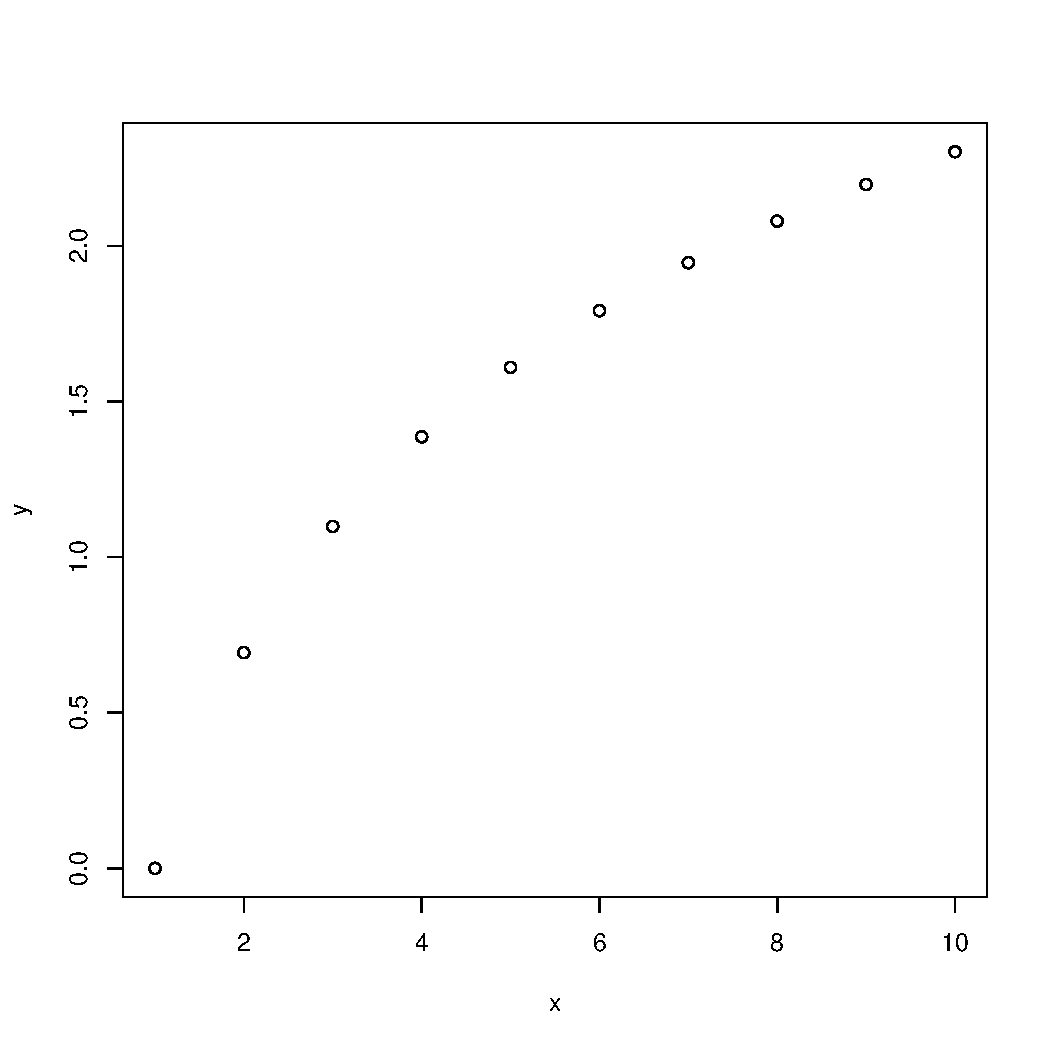
\includegraphics[width=0.75\textwidth]{Rplots.pdf}\end{figure}

\subsection{Table}

\LaTeX\ can be used to create tables\index{Tables}.

\begin{table}[H]
   \caption{Outcome matrix%
            \label{tab:OutcomeMatrix}}
   \begin{center}
      \begin{tabular}{|c|c||c|c|}
         \hline
         \multicolumn{2}{|c||}{} & \multicolumn{2}{c|}{\textbf{Unknown truth}} \\
         \cline{3-4}
         \multicolumn{2}{|c||}{} & $H_{0}$ & $H_{1}$ \\
         \hline \hline
                            &       &  correct                  & type II error \\
         \textbf{Decission} & $H_0$ & $\Pr=1-\alpha$            & $\Pr=\beta$ \\
                            &       & \emph{significance level} & (\emph{false negative}) \\
         \cline{2-4}
                            &       & Type I error              & Correct \\
                            & $H_0$ & $\Pr=\alpha$              & $\Pr=1-\beta$ \\
                            &       & (\emph{false positive})   & \emph{power of the test} \\
         \hline
      \end{tabular}
   \end{center}
\end{table}

\begin{table}[h]
 \centering
 \begin{tabular}{|l|r|r|r|}\hline
  Jaar&	Jongens&	Meisjes&	Totaal\\\hline
  1850&	67.240& 	64.176& 	131.416\\\hline
  1900&	99.026& 	94.204& 	193.230\\\hline
  1950&	73.354& 	69.616& 	142.970\\\hline
  2000&	58.790& 	56.093& 	114.883\\\hline
 \end{tabular}
 \caption{Geboortecijfers van Belgi\"e}
 \tiny{\url{http://statbel.fgov.be/nl/statistieken/cijfers/bevolking/geboorten\_vruchtbaarheid/}}
\end{table}

\subsection{Lists}

\subsubsection{Enumerate}

\begin{enumerate}
   \item First
   \item Second
   \item Third
\end{enumerate}

\subsubsection{Itemize}

\begin{itemize}
   \item First
   \item Second
   \item Third
\end{itemize}

\subsubsection{Descrioption}

\begin{itemize}
   \item[A] First
   \item[B] Second
   \item[C] Third
\end{itemize}

\subsubsection{Listing}

Listing like programming code can be included using the \texttt{verbatim}
environment.

\begin{verbatim}
x<-seq(0,10,0.1)
y<-log(x)
plot(x,y)
\end{verbatim}

Using the \texttt{lstlisting} environment from the \textbf{listings} package
programming code can be displayed in a more fancy way. 

\begin{lstlisting}[language=R]
x<-seq(0,10,0.1)
y<-log(x)
plot(x,y)
\end{lstlisting}

\appendix

\newpage
\section{Appendix A}

This is appendix A.

\section{Index}

\printindex

\end{document}
